\section{Statistics}

\subsection{Casual Inference}

La inferencia causal es el proceso de determinar el \textbf{efecto independiente de una variable} en un sistema más complejo. En general, este proceso es necesario cuando buscamos obtener conclusiones de datos pasados y en los que no es posible realizar un \textit{A/B testing}.

Existen 3 desafíos al realizar este proceso: 
\begin{itemize}
    \item \textbf{Cofounders}: Son aquellas variables que tienen un impacto en el \textit{outcome} y que incluso podrían tener un impacto en otras variables. 
    \item \textbf{Selection Bias}: Selección no representativa del grupo de control y tratamiento.
    \item \textbf{Counterfactuals}: Imputar valores en el grupo de control y tratamiento en base a \textit{Machine Learning} o algoritmos de \textit{Matching}. 
\end{itemize}

\begin{figure}[H]
    \center
    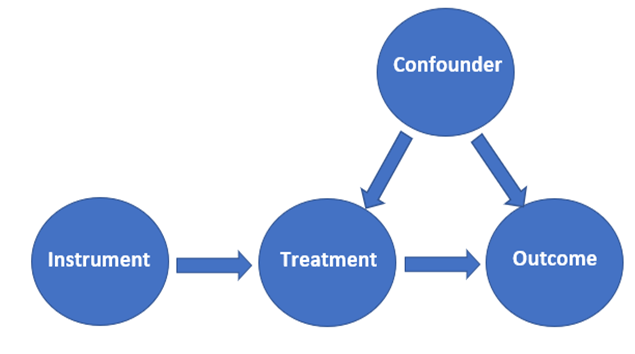
\includegraphics[scale=0.3]{notebooks/STATS/img/casual_inference_diagram.png}
    \caption{Casual Inference - DAG Diagram}
\end{figure}

Para resolver este problema, es necesario tomar algunos supuestos: 
\begin{enumerate}
    \item \textbf{Causal Markov Condition}: La influencia de las variables y el \textit{outcome} puede ser representado a través de un \textbf{Grafo Acíclico Dirigido (DAG)} en el que se asume la \textbf{condición de Markov}, es decir si $Y \rightarrow S \rightarrow C$, podemos asumir que $C \indep Y | S$
    \item \textbf{SUTVA}: (Stable Unit Treatment Value Assumption) El grupo de control y tratamiento \textbf{no tiene influencia el uno con el otro}. 
    \item \textbf{Ignorability}: Se excluye el ruido proveniente de cualquier otra fuente. 
\end{enumerate}

Consideremos el siguiente ejemplo 









